\documentclass[10pt, a5paper, twoside]{NGPLS}
\author{周造麟}
\title{30 天 LaTeX}

\usepackage{luatexja-fontspec}
\setmainjfont{jf-openhuninn-1.1.ttf}

\setlength{\parindent}{0pt}
\linespread{1.35}
\pagenumbering{arabic}

\usepackage[pipeTables, strikeThrough = true]{markdown}
\markdownSetup{fencedCode = true}
\markdownSetup{
  renderers = {
    image = {\begin{figure}[!htb]
      \centering
      \includegraphics[width = .8\linewidth]{#3}%
      \ifx\empty#4\empty\else
        \caption{#4}\label{fig:#1}%
      \fi
    \end{figure}},
    }
}
\usepackage{graphicx}
\graphicspath{{fig/}}

\usepackage{etoolbox}
%\AtBeginEnvironment{itemize}{\vskip6pt}
\AtBeginEnvironment{tabular}{\vskip6pt}
\AfterEndEnvironment{tabular}{\vskip6pt}

\usepackage[svgnames]{xcolor}
%\definecolor{LightGray}{gray}{0.9}

\usepackage{minted}
%\usemintedstyle{borland}

\usepackage{xurl}
\usepackage[breaklinks=true]{hyperref}
\urlstyle{same}
\hypersetup{
colorlinks=true,
linkcolor=blue,
urlcolor=cyan,
hyperindex = false
}

%\setlength{\parskip}{0.1\baselineskip}

\usepackage{amsmath}
\usepackage{amsfonts}
\usepackage{amssymb}

\usepackage{geometry}
\geometry{top=1.5cm, outer=1.75cm, inner=1.5cm, bottom=1.5cm, footskip=24pt}

\begin{document}%\color{Gold}\pagecolor{black}
\maketitle
\tableofcontents\newpage
\input{1拷貝}\newpage
\input{2拷貝}\newpage
\begin{markdown}
#30天 LaTeX 挑戰 Day 3 Overleaf

------

由於小弟我是使用 MacOS 所以我並不熟悉如何在 Windows 上建構環境,所以我在這裡介紹一個提供線上編譯 LaTeX 的網站 「***Overleaf***」,這樣既避免了操作系統上的差異,更可以像 Google Doc 一樣與他人共同編輯一個檔案。

##簡介

先前往 Overleaf 的網站 <https://www.overleaf.com>,你應該會看到與下圖一樣的畫面。

![Overleaf1](Overleaf1 "首頁") 

直接從下面的欄位註冊後應該會直接進到 Project 頁面,這裡是管理你的 Project 的地方,可以用旁邊的 New Project 按鈕新增新的 Project,除了創建一個空白的 Project 外也可以從 Github 匯入,甚至可以利用他人寫好,並在 Overleaf 上公開的模板,這也可以說是 Overleaf 中最方便的功能了。

![Overleaf3](Overleaf3 "Project 頁面")

創建新的 Project 或點進一個現有的 Project 後應該會看到與下圖一樣的畫面,在最左邊的上半部分是 Project 內所有的檔案,上面還有三個圖案,從左到右分別是創建新檔、新資料夾與上傳檔案。

![Overleaf4](Overleaf4 "點進 Project 後")

在這三個按鈕的上方是 menu ,點開後可以下載原始檔或編譯後的 PDF 檔,也可以調整一些有關 LaTeX 的設定,這裡介紹兩個重要的設定 Compiler 與 TeX Live Version,Compiler 就是編譯引擎加上格式,目前 Overleaf 支持 XeLaTeX, LaTeX, pdfLaTeX, LuaLaTeX,實際上還可以使用更多,但這就牽扯到 Overleaf 的底層了, TeX Live Version 是指定 TeX Live 的年份,這個選項會牽扯到 package 的版本,進而對輸出產生影響。

中間與右邊佔最大篇幅的是編輯器與 Pdf 瀏覽器,如果在 Pdf 瀏覽器上點兩下可以直接跳到相對應的原始碼區,而在 Pdf 瀏覽器上有一個綠色的按鈕,那就是最重要的編譯鈕,點下去後 Overleaf 就會開始編譯並產出 Pdf 檔。

##更多

當然,Overleaf 可以做的比這些還要多更多,詳細可以參考這些延伸文章,我最喜歡 Overleaf 的一點是他們很注重在使用體驗上,他們一直有在做使用者使用體驗調查,想盡辦法的提升使用者的感受。

不過如果你覺得 Overleaf 再怎麼好用也比不過本地的環境的話,可以參考這一篇來安裝,如果有遇到什麼問題也歡迎在下面留言詢問。

\end{markdown}\newpage
\input{4拷貝}\newpage
\begin{markdown}
#30天 LaTeX 挑戰 Day 5 使用前須知

-----

## 編譯檔案後

在 LaTeX 編譯完後會產生一些中間文件,這些中間文件可以依據功能不同分成以下幾種

* .log 編譯的紀錄檔,所有編譯中出現的問題都可以在這裡找到。
* .aux/.out 用來存放交叉引用的資料。
* .toc/.lof/.lot 目錄、表目錄、圖目錄的生成資料。
* .bbl/.bcf/.blg 與 biblatex 相關的文件。

如果編譯後發現突然多了許多檔案不要驚慌,這些都是 LaTeX 工作所需的檔案。

## 保留字符
下表為 LaTeX 中的保留字符

| 保留字符 | 用途 | 文檔中使用 | 替代指令 |
| :-------- | :---- | :----- | :----- |
|\ |所有命令的開頭|\$\backslash\$|\textbackslash|
|{|開始一個分組|\\{|\textbraceleft|
|}|結束一個分組|\\}|\textbraceright|
|\$|進入數學模式|\\$|\textdollar|
|%|下註解|\\%|NA|
|#|定義巨集|\\#|NA|
|&|表格中的換格標示|\\&|NA|
|\_|數學模式下產生下標字|\\_|\textunderscore|
|^|數學模式下產生下標字|\\^|\textasciicircum|
|~|產生一個空白(禁止斷行)|\\~|\textasciitilde|

大部分的保留字符都可以藉由加一個反斜槓的方式輸出,但唯有反斜槓不行(單個反斜槓是產生空白、兩個反斜槓加在一起是強制換行)只能使用指令 \textbackslash 來輸出。

### 分組

分組是 LaTeX 中的一個概念,可以將其類比為一個 HTML 的 \<p\> 標籤,通常用來限定命令的作用範圍,使用方式也很簡單,就是將想讓命令作用的範圍用{包起來就好了},範例如下。

```latex
\large %更改字型大小
{\large A}A
```
應該會得到下圖的結果
<圖片>
## 命令與環境

命令與環境的差別差在哪裡?相信這是大家最想問的,你可以將命令理解為由反斜槓開始直到數字、保留字符或空白的字串,將環境理解為被 \begin{環境}......\end{環境} 包裹著的區塊,而實際上環境更像是將開啟一個分組與一連串命令加在一起。

```latex
%以下兩種方式在編譯後都會得到一樣的結果
{\large 放大}\begin{large}放大\end{large}
```

### 假空白

LaTeX 的命令有可分為兩種有參數與沒參數的,通常可選參數會被 [] 包圍起來並置於被 {} 包圍起來的的必選參數前。前面提到命令只會在遇到數字、保留字符或空白才會被視為一個整體,這就會導致一個問題,像 `\LaTeX` 這樣沒有必選參數的命令後面必須要接一個空白,但這個空白會被 LaTeX 忽略掉,導致下面的情況

<圖片>

以下有兩個可以解決這個問題的方法

```latex
\LaTeX{}%在命令後接花括號

\LaTeX\ %在命令之後接反斜槓
```

## 處理錯誤

LaTeX 的錯誤有下列三種

* warning
* badbox
* error

第一種是 warning 代表發生了錯誤但並不影響、或不太影響排版結果的問題上,通常這種回去翻 log 檔都會有一些建議,不過不解決也不會什麼大事情發生。

badbox 是 LaTeX 的一個特殊的錯誤類型,這個錯誤類型是來自於 LaTeX 認為排版產出的結果不美觀,而給出的警告,在這類的警告後面通常還會有 badness 來描述到底有多糟糕。

error 則與 warning 相反,其足以使編譯過程停止或導致奇怪的結果,遇到這種問題建議直接向他人詢問,並請附上原始檔與 log 檔的紀錄,以便他人快速釐清問題所在。

\end{markdown}\newpage
\input{6拷貝}\newpage
\input{7拷貝}\newpage
\input{8拷貝}\newpage
\input{9拷貝}\newpage
\begin{markdown}
#30天 LaTeX 挑戰 Day 10 圖片

------

LaTeX 本身是不能處理圖片的,所以我們需要借用 graphicx 來讓 LaTeX 處理圖片,其實還有另一個可以處理圖片的 package 叫 graphics ,他們兩個像是同一個 package 但用著不同的 interface ,兩個除了可選參數的形式之外,不論是命令還是必選參數都一樣。在這裡介紹的是 graphicx ,如果想要使用 graphics 請參考說明文件<連結>

##基礎

只要使用`\includegraphics{檔案}`就可以將圖片導入文件中了

```latex
\includegraphics{test.png}
```

但這樣會有一個問題,如果今天圖片與 tex 檔不在同一層目錄下就找不到,圖片少的時候還好,但只要圖片一多再加上 LaTeX 編譯時產生的中間文件就足以將你淹沒在茫茫檔案之中,萬幸的是可以利用`\graphicspath{目錄}`來指定圖片檔案的位置。

```latex
\graphicspath{{jpg/}{png/}}
```

這樣 LaTeX 就會自動搜尋 jpg 跟 png 的子目錄了,你可以利用以下的可選參數來調整圖片

|參數|含義|
|-----|-----|
|scale|圖片縮放|
|width|圖片寬度|
|height|圖片高度|
|page|如果是插入多頁pdf,要插入第幾頁|
|draft|啟動草稿模式|

```latex
\includegraphics[scale=0.25]{test.png}\\
\includegraphics[scale=0.5]{test.png}\\
\includegraphics[scale=0.75]{test.png}\\
\includegraphics[draft]{test.png}
```

###除了圖片之外

除了圖片外 graphicx 也提供了以下指令

* `\rotatebox{角度}{文字}`
* `\scalebox{水平縮放}[垂直縮放]{文字}`
* `\reflectbox{文字}`

第一個 `\rotate{}{}` 顧名思義就是旋轉文字

```latex
\rotatebox{0}{文字}\\
\rotatebox{90}{文字}\\
\rotatebox{180}{文字}\\
\rotatebox{270}{文字}\\
```

第二個 `\scalebox{}[]{}` 可以將文字做兩個不同方向的縮放,第三個 `\reflectbox{} `則是讓文字左右翻轉,實際上可以看成 `\scalebox{-1}[1]{文字}`的簡寫

```
\scalebox{1}[1]{文字}\\
\scalebox{2}[1]{文字}\\
\scalebox{1}[2]{文字}\\
\scalebox{2}[2]{文字}\\
\scalebox{-1}[1]{文字}\\
\reflectbox{文字}
```

##浮動體環境

按著以上的方式用了一段時間後,你可能會發現這樣產出的結果並不好看,這時只要將圖片放進 figure 環境即可,LaTeX 就會自動幫挑選好位置插入圖片了

```latex
\begin{figure}
\includegraphics[scale=0.5]{test.png}
\end{figure}
```

你會發現插入圖片的位置跟程式碼的位置不太一樣,這是因為 LaTeX 會自動決定他認為好看的位置,而不是我們想要的位置,這時候可以在 `\begin{figure}[]`後的方括號加入參數

|參數|含義|
|-----|-----|
| h |將圖片放在這裡(不一定跟程式碼一樣,但會相近)|
| t |放在頁面頂部|
| b |放在頁面底部|
| p |為圖片單獨開一頁|
| ! |覆蓋 LaTeX 預設用來決定「好」位置的參數|

```latex
\begin{figure}[h]
\includegraphics[scale=0.5]{test.png}
\end{figure}
```

###文繞圖

如果你想要達成文繞圖的效果,需要借助 wrapfig package 提供的 wrapfig 環境

```latex
%\begin{wrapfigure}{位置}{寬度}
\begin{wrapfigure}{r}{6cm}
\includegraphics[width=5.5cm]{test.png}
\end{wrapfigure}
```

下表是可以使用的位置

|參數|含義|
|-----|-----|
| r |靠右側|
| l |靠左側|
| i |雙面模式下靠書封|
| o |雙面模式下靠書的開口|

\end{markdown}\newpage
\input{11拷貝}\newpage
\begin{markdown}
#30天 LaTeX 挑戰 Day 12 xcolor

------

在前半段的使用中 LaTeX 產出的文字都是黑白的,如果想要讓 LaTeX 變成彩色的,需要加入 xcolor 這個 package

##定義顏色

xcolor 提供了`\definecolor{名字}{模型}{參數}` 命令供定義顏色,xcolor 支持 html, rgb, cmyk 等等的顏色模型,用不同的模型會影響參數的形式,

```latex
\definecolor{cyan1}{rgb}{0, 255, 255}
\definecolor{cyan2}{html}{00FFFF}
\definecolor{cyan3}{cmyk}{255, 0, 0, 0}
```

上面雖然都用不同的顏色模型,但定義出的顏色都是一樣的,xcolor 本身有預定義一些基本顏色,如同下圖所示

<圖片>

除此之外 color 也提供了`svgnames, dvinames, x11names` 這三個選項提供更多預定義好的顏色

```latex
\usepackage[svgnames]{xcolor}
\usepackage[dvinames]{xcolor}
\usepackage[x11names]{xcolor}
```

如果想要讓兩種顏色混合,可以利用`\colorlet{名稱}{混合方式}`來混合兩種顏色


```latex
\colorlet{mycolor1}{yellow!10!red}
\colorlet{mycolor2}{blue!10}
```

mycolor1 會是 10\%的黃色加上90\%紅色,mycolor2 會是10\%藍色加上90\%的白色。

##文字顏色

想要讓文字上色有兩種辦法,一種是利用`\color{}`將更改預設顏色,另一種是利用`\textcolor{顏色}{文字}`小範圍的更改。

```latex
\color{yellow}
Banana\\
\color{red}
Apple \textcolor{blue}{Ocean}
```

如果是想要幫文字上底色,可以使用`\colorbox{顏色}{文字}`上色

```latex
|\colorbox{yellow}{Important}|
\colorbox{yellow}{Important}
```

如果想要邊匡,可以利用`\fcolorbox{邊匡顏色}{底色}{文字}`

```latex
\colorlet{mycolor}{blue!50}
\fcolorbox{red}{yellow}{IMPORTANT}\\
\fcolorbox{blue}{mycolor}{Relax}
```

##背景顏色

背景顏色可以利用`\pagecolor{}`來更改

```latex
\pagecolor{red}
A red paper with some message.
```

\end{markdown}\newpage
\begin{markdown}
#30天 LaTeX 挑戰 Day 13 交叉引用

-------

在寫文章時,如果遇到要引用到文章前面的狀況往往是最讓人頭疼的,因為只要文章一被改過,你就很有可能需要將後面引用到的部分全部修改過,幸好 LaTeX 針對這個問題提供了`\label{}, \ref{} &\pageref{}`這三個指令,拯救我們脫離水深火熱之中。

##引用章節

`\label{}` 顧名思義就是在文章中放入一個標籤,等到需要時再利用`\ref{} 或 \pageref{}` 來引用

```latex
\section{原子說}\label{sec:Atomic Theory}
假文假文假文假文假文假文假文假文假文假文假文假文假文假文假文假文假文假文假文假文假文假文假文假文假文假文假文假文假文假文假文假文假文假文假文

\section{定比定律}
根據第\ref{sec:Atomic Theory}章的內容⋯⋯
```

如果你想把頁碼一起含進去,可以使用`\pageref{}`來完成

```latex
\section{原子說}\label{sec:Atomic Theory}
假文假文假文假文假文假文假文假文假文假文假文假文假文假文假文假文假文假文假文假文假文假文假文假文假文假文假文假文假文假文假文假文假文假文假文

\section{定比定律}
根據第\pageref{sec:Atomic Theory}頁第\ref{sec:Atomic Theory}章的內容⋯⋯
```

##引用表格 & 引用圖片 & 引用方程式

想要引用這三種元素很簡單,只需要將`\label{}`放入環境之中即可

```latex
\begin{figure}[h]\label{fig:1}
\includegraphics{Triangle.png}
\end{figure}
圖\ref{fig:Triangle}是一個三角形\\

\begin{tabular}{|c c c|}\label{tab:1}
\hline
$\theta^\circ$ & $\sin(\theta^\circ)$ & $\cos(\theta^\circ)$\\
\hline
$30^\circ$ & $\frac{\sqrt{3}}{2}$ & $\frac{1}{2}$\\
$45^\circ$ & $\frac{\sqrt{2}}{2}$ & $\frac{\sqrt{2}}{2}$\\
$60^\circ$ & $\frac{1}{2}$ & $\frac{\sqrt{3}}{2}$\\
\hline
\end{tabular}

表\ref{tab:sin}是角度與$\sin, \cos$值的關係表

\begin{equation}\label{eq:1}
a^2 + b^2 = c^2
\end{equation}
方程式(\ref{eq:1})是畢氏定理
```

需要注意的是如果環境內有`\caption{}`命令,建議將`\label{}`命令放在`\caption{}`後。

##其他元素

如果你想要引用的是自定義的編號環境,引用方式就如同引用 LaTeX 內建的環境一樣,但如果你想要引用的元素並不是以上這幾種,那你可以考慮直接用`\pageref{}`引用頁碼。

##超連結

你會注意到引用雖然好用,但沒有辦法點下去前往被引用的元素,這時後我們可以利用 `hyperref` 這個 package 來救場。

```latex
\section{原子說}\label{sec:Atomic Theory}
假文假文假文假文假文假文假文假文假文假文假文假文假文假文假文假文假文假文假文假文假文假文假文假文假文假文假文假文假文假文假文假文假文假文假文

\section{定比定律}
根據第\pageref{sec:Atomic Theory}頁第\ref{sec:Atomic Theory}章的內容⋯⋯
```

你可以看到在`\pageref{}`產生的數字上出現了紅匡,且點下去會前往被引用的區段,但除了這之外,`hypperef` 也提供了 `\href{連結}{顯示文字}`與`\url{連結}`來在文件中插入超連結

```latex
\href{https://www.overleaf.com}{Overleaf}\\
\url{https://www.overleaf.com}
```

如果你不喜歡連結被紅匡包起來,可以利用`\hypersetup{}`來更改

```latex
\hypersetup{hidelinks}
\href{https://www.overleaf.com}{Overleaf}\\
\url{https://www.overleaf.com}
```

這裡有可以更改的參數

|參數|含義|值|
|------|------|------|
|linkcolor|內部連結顏色|顏色名字|
|urlcolor|超連結顏色|顏色名字|
|colorlinks|是否幫連結上色|布林值|
|breaklinks|是否允許連結換行|布林值|
\end{markdown}\newpage
\input{14拷貝}\newpage
\begin{markdown}
#30天 LaTeX 挑戰 Day 15 數學(下)

------

今天的內容有涉及到美國數學家協提供的 **amssym, amsfonts** 與 **amsmath** ,若有涉及到這些 package 的應用,我會在下面特別標注,如果沒有標註就是 LaTeX 基本的使用。

##各種的應用

基本的函數都是用反斜槓加函數名稱的方式輸出

||||
|------|------|------|------|
|\sin |\cos |\tan |\cot |
|\arccos |\arcsin |\arctan |\sec |
|\csc |\exp |\log |\deg |
|\lim |\inf |\min |\max |

想要使用其他字體嗎?LaTeX 提供了以下幾種字體

|字體|結果|
|-----|-----|
|`\mathrm{ABCabc123}`|$\mathrm{ABCabc123}$|
|`\mathit{ABCabc123}`|$\mathit{ABCabc123}$|
|`\mathnormal{ABCabc123}`|$\mathnormal{ABCabc123}$|
|`\mathcal{ABCabc123}`|$\mathcal{ABCabc123}$|

數學模式的輸出皆為斜體,可以用 `\mathrm{}` 轉為正體,如果想在數學模式中加粗字體,可以利用 **amsmath** 提供的 `\boldsymbol` 命令

```latex
$
\mu ,\boldsymbol{\mu}\\
\delta ,\boldsymbol{\delta}
$
```

空心粗體則需要 amsfonts 提供的 `\mathbb{}` 命令

```latex
$
x > 1 and x \in \mathbb{R}
$
``` 

如果想要將某個公式的推導過程寫下,可以利用 **amsmath** 提供的 align 環境

```latex
\begin{align}

\end{align}
```

在想要對齊的地方用 & 指定即可,實際上的使用方式就與表格類似,如果不想要編號,使用帶星號的 `align*` 即可

```latex
\begin{align*}

\end{align*}
```

如果需要輸出矩陣,可以使用 `matrix` 環境

```latex
$
\begin{matrix}
3 & 0\\
0 & 3
\end{matrix}
$
```

但這樣就只是一些對齊的的數字,所以我們可以利用以下的方式來輸出含有小括號的矩陣

```latex
\[
\left(\begin{matrix}
2 & 0\\
0 & 2
\end{matrix}\right)
\]
```

或者使用由 **amsmath** 提供的 pmatrix 環境

```latex
\[
\begin{pmatrix}
2 & 0\\
0 & 2
\end{pmatrix}
\]
```

不只是小括號,也可以使用方括號、花括號

```latex
\[
\begin{bmatrix}
2 & 0\\
0 & 2
\end{bmatrix}
\begin{Bmatrix}
2 & 0\\
0 & 2
\end{Bmatrix}
\]
```

甚至是行列式也可以利用這個方法輸出

```latex
\[
\begin{vmatrix}
2 & 0\\
0 & 2
\end{vmatrix}
\begin{Vmatrix}
2 & 0\\
0 & 2
\end{Vmatrix}
\]
```

如果想要輸出聯立方程式,可以利用 **amsmath** 提供的 cases 環境

```latex
\[
\begin{cases}
x &= 1\\
y &= 3x + 9
\end{cases}
\]
```

當然,我所列出的例子只是滄海一粟,實際上還有更多的可能性,但由於我很少利用這部分的功能,所以我只能簡單地把我知道的使用方式全都寫出,更進一步的使用方式可以參考這些文章。

\end{markdown}\newpage
\begin{markdown}
#30天 LaTeX 挑戰 Day 16 化學相關

------

LaTeX 也能拿來排版化學相關的事物,但我們需要借用 mhchem 與 chemfig 的力量

```latex
\usepackage{mhchem}
\usepackage{chemfig}
```

##化學式 & 化學反應式

化學式與化學反應式利用 mhchem 提供的`\ce{}`就可以達成了

```latex
\ce{H2O}\\
\ce{H2O2}\\
\ce{NO-}
```

如果需要質量數可以用以下的方式

```latex
\ce{^235_98U}\\
\ce{^2_1H}\\
\ce{^4_2He}
```

`^`代表上標`_`代表下標,也可以打出分子內離子的氧化態

```latex
\ce{Fe^{II}Fe^{III}2O4}
```

計量化學也可以利用相同的方式

```latex
\ce{2H2O}\\
\ce{1/2H2O}\\
\ce{(1/2)H2O}\\
\ce{$n$H2O}
```

化學反應式只需要加入`+`或`->`等等就好了

```latex
\ce{H2O2 -> H2O + O2}
```

如果涉及到沈澱或產生氣體可以利用單獨的`^`跟單獨的小寫 v,可逆反應則更改箭頭的樣式即可

```latex
\ce{^ v}\\
\ce{A <=> B}\\
\ce{CaCO_3 + HCl <=> CaCl_2 v + H_2O + CO_2 ^}
```

如果需要加催化劑,可以用箭頭後加中括號的方式達成

```latex
\ce{A ->[text above][text below] B]}\\
\ce{H2O2 ->[MnO2] H2O + O2 ^}\\
$\ce{x Na(NH4)HPO4 ->[\Delta] (NaPO3)_x + x NH3 ^ + x H2O}$
```

下圖是 mhchem 可以使用的箭頭種類

<圖片>

##結構式

結構式需要借助 chemfig 提供的`\chemfig{}`命令

```latex
\chemfig{H-O-H}
```

你可能會想要調整角度,在`-`後加[]可以解決這個問題,chemfig 可以接受預設角度、絕對角度與相對角度的輸入,預設角度就直接在括號內加入數字,預設是 0 ,之後每增加 1 角度增加 45 度,絕對角度需要在數字前加入`:`,相對角度則是加入`::` 

```latex
\chemfig{A-[1]-[2]-[3]-[4]-[5]-[6]-[7]-[8]}
\chemfig{A-[:45]-[:90]-[:135]-[:180]-[:225]-[:270]-[:315]-[:360]}
\chemfig{A-[::+45]-[::+45]-[::+45]-[::+45]-[::+45]-[::+45]-[::+45]-[::+45]}
```

如果想要畫多邊形可以利用下面的技巧

```latex
\chemfig{C*5(-A-B-C-D-E-F)}\\
\chemfig{[:18]C*5(-A-B-C-D-E-F)}
```

如果你真的想做點什麼複雜的東西,我建議你可以參考奈米小人

\end{markdown}\newpage
\begin{markdown}
#30天 LaTeX 挑戰 Day 17 listing

------

如果在 LaTeX 想要輸出程式碼,顯然不可能用 `\textbackslash LaTeX`  如此陽春的方法,所以我們需要特殊的環境或 package 來達成目的。

##verb

最陽春的方法就是利用 LaTeX 內建的 `\verb|......|` 來輸出在行內的程式碼

```latex
用 \verb|\begin{center}| 來將文字置中
```

如果是很重要的程式碼,你想專門為他開一個區塊,可以利用 `\begin{verbatim}......\end{verbatim}` 環境

```latex
\begin{verbatim}
\newcounter{example}
\newenvironment{example}{\refstepcounter{example}\textbf{Example.\theexample}\ }{\\}
\end{verbatim}
```

可以看到這一段程式碼單獨的獨立了出來。

##listings

但這樣並不會幫程式碼上色,如果想要美觀的的輸出程式碼可以借助 listings package 的協助。

```latex
\begin{lstlisting}
\begin{itemize}
\item 1
\item 2
\item 3
\end{itemize}
\end{lstlisting}
```

你會看到上面的例子也沒有改善多少,這是因為我們還沒設定程式碼應該長怎樣。

```latex
\begin{lstlisting}[language={[LaTeX]TeX}, commentstyle=\color{red} ,keywordstyle=\color{blue}, numbers=center]
\begin{itemize}
\item 1
\item 2
\item 3
\end{itemize}
%一個不知道為什麼的列表
\end{lstlisting}
```

這樣看起來就好許多了,可是每一次都打這一大長串也不方便,所以可以利用 `\lstset `來設定默認的參數。

```latex
\lstset{
    language={[LaTeX]TeX},
    basicstyle=\sffamily,
    numbers=left,
    numberstyle=\scriptsize,
    frame=tb,
    tabsize=4,
    commentstyle=\color{blue},
    keywordstyle=\color{red},
    morekeywords={ce,draw,node,foreach,in,chemfig,bond,href,hologo,
    ifthenelse,addplot,addplot3,coordinates}
}
```

language 是設定程式語言的類型,basicstyle 是設定列出來成果的格式,numberstyle 是控制數字的格式,commentstyle 是控制註解的格式,keywordstyle 是控制關鍵字的格式,morekeywords 則是可以自行加入星的關鍵字。

##minted

但上面的方法有一個問題,就是他只能標記出有被設定過的關鍵字,有時候多少會有點不方便,於是有人將 Pygment 與 LaTeX 結合起來做成了 minted 這個 package,在使用 minted 之前請先確保自己的電腦內有 Pygment詳細的下載方式請參考下面這篇文章。<https://clay-atlas.com/blog/2020/02/10/python-chinese-tutorial-package-pygments-code-highlight/>

minted 提供了 `\begin{minted}[參數]{語言}......\end{minted}` 來輸出程式碼

```latex
\begin{minted}{latex}
\begin{itemize}
\item 1
\item 2
\item 3
\end{itemize}
\end{minted}
%一個不知道為什麼的列表
```

可以看到這樣好看很多,如果想要微調輸出格式可以在利用以下的參數。

|參數|含義|
|------|------|
|lineos|顯示程式碼行數|
|bgcolor|背景顏色|
|numbers|顯示程式碼行數(可指定位置)|
|mathescape|可以在 minted 環境中直接輸入數學方程式|
|escapeinside|設定跳拖字符|
|breaklines|可不可將程式碼換行|

```latex
\begin{minted}[lineos, breaklines, mathescape, escapeinside=| |]{latex}
\begin{itemize}
\item 1
\item 2
\item 3
\end{itemize}
$\Sigma_{k=100} \sin(k^\circ)$
|\textcolor{red}{ABC}|
\end{minted}
```

如果想要使用別種配色,Pygment 有內建許多不同的 style 可供選擇,只要使用`\usemintedstyle{style}` 選擇即可。

```latex
%\usemintedstyle{vim}
\begin{minted}[lineos, breaklines, mathescape, escapeinside=| |]{latex}
\begin{itemize}
\item 1
\item 2
\item 3
\end{itemize}
$\Sigma_{k=100} \sin(k^\circ)$
|\textcolor{red}{ABC}|
\end{minted}
```

這樣就可以更改樣式了,詳細的樣式與支持的語言,請參考 Pygment 的官網。

\end{markdown}\newpage
\begin{markdown}
#30天 LaTeX 挑戰 Day 18 tcolorbox

------

今天要介紹的是 tcolorbox,它提供了一個簡單的產生高度客製化 color box 的方式。

##基礎使用

tcolorbox 提供了`tcolorbox`這個環境供我們建立 colorbox

```latex
\begin{tcolorbox}
This is a colored box.
\end{tcolorbox}
```

###Style

|參數|含義|
|-----|-----|
|colback|底色|
|colbacklower|下半部分的底色|
|colframe|邊匡顏色|
|coltitle|title 欄的底色|
|colupper|上半部分文字的顏色|
|collower|下半部分文字的顏色|
|coltext|文字顏色|
|subtitle style|title 欄的樣式|
|boxrule|邊匡粗細|
|fonttitle|標題文字的樣式|
|fontupper|上半部分文字的樣式|
|fontlower|下半部分文字的顏色|

需要注意的是`colbacklower`需要搭配其他命令才可使用,之後會介紹到,如果想要設定一個預設值可以利用`\tcbset{}`來完成。

###標題與副標題

可以用`[title=title]`為他加入標題

```latex
\begin{tcolorbox}[title=Title]
This is a colored box with a title.
\end{tcolorbox}
```

也可以用`\tcbsubtitle{Subtitle}`來插入副標題

```latex
\begin{tcolorbox}[title=Title]
This is a colored box with a title.
\tcbsubtitle{Subtitle}
And subtitle.
\end{tcolorbox}
```

###上下分段

如果你想要將一個 box 分成兩段可以利用`\tcblower` 

```latex
\begin{tcolorbox}
Upper Box
\tcblower
Lower Box
\end{tcolorbox}
```

這樣預設會是上下兩段,可以利用`sidebyside`改成左右各佔一半

```latex
\begin{tcolorbox}[sidebyside]
Upper Box
\tcblower
Lower Box
\end{tcolorbox}
```

###更多

但 tcolorbox 可不只有這樣,你可以利用`\tcbuselibrary{}`去調用一些延伸功能,例如調用 skin 可以讓上下兩段的顏色分開設定

```latex
%\tcbuselibrary{skins}
\begin{tcolorbox}[skin=bicolor, sidebyside, colback=gray!30!white,colbacklower=gray!5!white]
Bicolor
\tcblower
Bicolor
\end{tcolorbox}
``` 

當然除了上述的技巧之外,tcolorbox 還有許多用處我沒有講到,如果想要好好的研究可以參考他的使用手冊<連結>。

\end{markdown}\newpage
\begin{markdown}
#30天 LaTeX 挑戰 Day 19 Ti*k*Z

-------

TikZ 是一個強大的繪圖 pacakge,幾乎可以畫出任何東西

##基礎使用

有兩種方式使用 TikZ 繪圖,第一是將命令放在 `\tikz `後,第二是將命令用放在 tikzpicture 環境中

```latex
\tikz 命令
\begin{tikzpicture}
命令
\end{tikzpicture}
```

###直線

在 Tikz 中畫直線需要用到`\draw[選項]`這個命令

```latex
\draw[選項] ...... ;
```

如果想要畫一條直線,只需要在`\draw `的後面加上點的座標標,再由\-\- 連起來即可,最後不要忘記加上分號

```latex
\tikz \draw (0,0)--(2,0)--(2,2);
```

我們可以將起點與終點的座標重疊,達成封閉圖形的效果

```latex
\tikz \draw (0,0)--(2,0)--(2,2)--(0,0);
```

但這樣會有一個問題,如果你加入 [rounded corners] 這個讓原本鋒利的邊角變成圓角的參數時,你就會發現有問題

```latex
\tikz \draw[rounded corners] (0,0)--(2,0)--(2,2)--(0,0);
```

這是因為圖片只有看起來是是封閉的,但 TikZ 並不認為他是一個封閉的圖形,這時候只需要在最後加入 `--cycle` 就可以避免這個問題了

```latex
\tikz \draw[rounded corners] (0,0)--(2,0)--(2,2)--cycle;
```

###矩形

畫矩形也可以用上面的方式畫,但 TikZ 有提供更簡單的方式

```latex
\tikz \draw (0,0) rectangle (2,2);
```

你只需要在 rectangle 後放入對腳座標即可

###圓形、橢圓形、圓弧

畫一個圓也非常簡單,先給出圓心再給出半徑,中間要加入 circle 將兩者隔開即可

```latex
\tikz \draw (0,0) circle (2);
```

在上圖中的是一個圓心在 (0,0) 半徑為 2 的圓形,畫橢圓形與畫圓形類似,只不過需要把 circle 換成 ellipse ,且在指定長軸與短軸時需用 and 將兩者隔開

```latex
\tikz \draw (0,0) ellipse (2 and 1);
```

圓弧則是將 ellipse 換成 arc ,並需要額外指定角度

```latex
\tikz \draw (0,0) arc (0:270:1);
```

上圖畫出了一個由 (0,0) 開始、從 0 度畫到 270 度、半徑為 1 的四分之三圓弧,橢圓形的圓弧當然也可以這樣畫出來

```latex
\tikz \draw (0,0) arc (0:270:1 and 2);
```

###曲線

曲線則是將直線中的`--`換成 .. 就可以畫出貝茲曲線,也因為是畫出貝茲曲線,所以需要加入至少一個控制點

```latex
\tikz \draw (0,0).. controls (1,1) ..(2,0);
```

多個控制點則需要用 and 區隔

```latex
\tikz \draw (0,0).. controls (0.5,1) and (1.5,1) ..(2,0);
```

###格線

格線則是利用 grid 來達成

```latex
\tikz \draw (0,0) grid (0.5,1) and (1.5,1) ..(2,0);
```

###極座標

除了平面座標外也可以指定極座標

```latex
\tikz \draw (0:0)--(45:1);
```

\end{markdown}\newpage
\begin{markdown}
#30天 LaTeX 挑戰 Day 20 Ti*k*Z

--------

##可用的選項

TikZ 提供了大量的可自定義的選項,供使用者畫出自己想像中的圖片

###顏色

顏色可以利用 draw 來決定

```latex
\draw[draw = blue] (0,0)--(5,0);
\draw[draw = red] (0,-1)--(5,-1);
\draw[draw = yellow] (0,-2)--(5,-2);
```

如果要填色,可以利用 fill 來填滿顏色,如果目前的圖形不是封閉圖形,那會自動變成封閉圖形

###粗細

粗細可以利用 line width 來決定

```latex
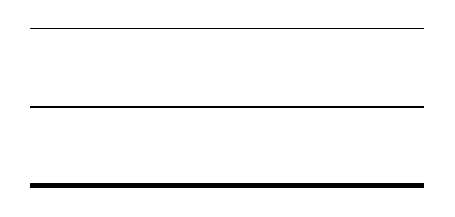
\begin{tikzpicture}
\draw (0,0)--(5,0);
\draw[line width = 1pt] (0,-1)--(5,-1);
\draw[line width = 2pt] (0,-2)--(5,-2);
\end{tikzpicture}
```

TikZ 的預設值是 0.4pt

###箭頭

可以利用 > 與 < 來指定箭頭的形式

```latex
\begin{tikzpicture}
\draw[-] (0,0)--(5,0);
\draw[<-] (0,-1)--(5,-1);
\draw[->] (0,-2)--(5,-2);
\draw[<->] (0,-3)--(5,-3);
\draw[|->] (0,-4)--(5,-4);
\draw[|<->|] (0,-5)--(5,-5);
\draw[|-|] (0,-6)--(5,-6);
\draw[->|] (0,-7)--(5,-7);
\draw[>->>] (0,-7)--(5,-7);
\end{tikzpicture}
```

上圖是一些示範

###預定義好的樣式

TikZ 也有預先定義好一些樣式,讓我們可以使用

```latex
\begin{tikzpicture}
\draw[dotted] (0,0)--(5,0);
\draw[densely dotted] (0,-1)--(5,-1);
\draw[loosely dotted] (0,-2)--(5,-2);
\draw[dashed] (0,-3)--(5,-3);
\draw[densely dashed] (0,-4)--(5,-4);
\draw[loosely dashed] (0,-5)--(5,-5);
\end{tikzpicture}
```

###平移、縮放與旋轉

可以利用 shift 來達成平移的效果

```latex
\begin{tikzpicture}
\draw (0,0) rectangle (1,1);
\draw[shift={(2,0)}] (0,0) rectangle (1,1);
\draw[shift={(2,2)}] (0,0) rectangle (1,1);
\draw[shift={(0,2)}] (0,0) rectangle (1,1);
\draw[shift={(-2,2)}] (0,0) rectangle (1,1);
\draw[shift={(-2,0)}] (0,0) rectangle (1,1);
\draw[shift={(-2,-2)}] (0,0) rectangle (1,1);
\draw[shift={(0,-2)}] (0,0) rectangle (1,1);
\draw[shift={(2,-2)}] (0,0) rectangle (1,1);
\end{tikzpicture}
```

* 第二個正方形的左下頂點由 (0,0) 移到了 (2,0)
* 第三個正方形的左下頂點由 (0,0) 移到了 (2,2)
* 第四個正方形的左下頂點由 (0,0) 移到了 (0,2)
* 第五個正方形的左下頂點由 (0,0) 移到了 (-2,2)
* 第六個正方形的左下頂點由 (0,0) 移到了 (-2,0)
* 第七個正方形的左下頂點由 (0,0) 移到了 (-2,-2)
* 第八個正方形的左下頂點由 (0,0) 移到了 (0,-2)
* 第九個正方形的左下頂點由 (0,0) 移到了 (2,-2)

也可以在 shift 前加上 x 或 y 來決定平移的方向,但在這種情況下就不能使用內建的長度單位,需要自行指定

```latex
\begin{tikzpicture}
\draw (0,0) rectangle (1,1);
\draw[xshift=100pt] (0,0) rectangle (1,1);
\draw[xshift=-100pt] (0,0) rectangle (1,1);
\draw[yshift=100pt] (0,0) rectangle (1,1);
\draw[yshift=-100pt] (0,0) rectangle (1,1);
\end{tikzpicture}
```

旋轉則需要利用 rotate

```latex
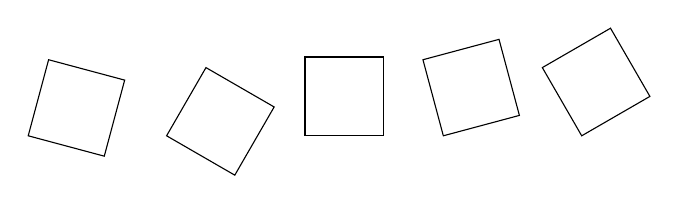
\begin{tikzpicture}
\draw (0,0) rectangle (1,1);
\draw[xshift=100pt, rotate=30] (0,0) rectangle (1,1);
\draw[xshift=50pt, rotate=15] (0,0) rectangle (1,1);
\draw[xshift=-100pt, rotate=-15] (0,0) rectangle (1,1);
\draw[xshift=-50pt, rotate=-30] (0,0) rectangle (1,1);
\end{tikzpicture}
```

\end{markdown}\newpage
\begin{markdown}
#30天 LaTeX 挑戰 Day 21 Ti*k*Z

-------

##進階使用

###節點

在 TikZ 中可以利用 `\node(name) at(x,y) {text};` 放置節點

```latex
\begin{tikzpicture}
\draw[help lines] (-2,-2) grid (2,2);
\node(1) at(0,0) {原點};
\end{tikzpicture}
```

想要連接兩個節點時,可以將座標改為兩個節點的名字

```latex
\begin{tikzpicture}
\node(A) at(0,0) {A};
\node(B) at(2,0) {B};
\node(C) at(0,2) {C};
\draw (A)--(B)--(C);
\end{tikzpicture}
```

`\node `如同 `\draw `也可以使用選項來調整樣式

```latex
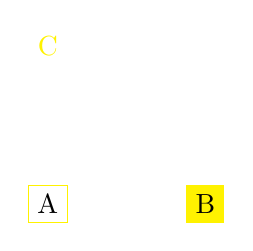
\begin{tikzpicture}
\node[draw=yellow](A) at(0,0) {A};
\node[fill=yellow](B) at(2,0) {B};
\node[text=yellow](C) at(0,2) {C};
\end{tikzpicture}
```

當然也有一些是只能用在 `\node `上的選項

```latex
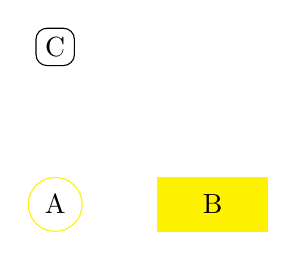
\begin{tikzpicture}
\node[draw=yellow,circle](A) at(0,0) {A};
\node[fill=yellow, minimum width=40pt, minimum height=20pt](B) at(2,0) {B};
\node[draw=black, rounded corners](C) at(0,2) {C};
\end{tikzpicture}
```

* 第一個節點用 circle 將外匡變成圓形的
* 第二個節點用 minimum width/height 定義節點的最小長寬
* 第三個節點用 rounded corners 把節點的邊角轉成圓角

但有時候我們並不想要直接把節點放到指定的座標,而是想放到該座標的上下左右,這個時候也可以利用 TikZ 內建的選項來達成

```latex

\begin{tikzpicture}
\node[left] at(0,0) {left};
\node[right] at(0,0) {right};
\node[above] at(0,0) {above};
\node[below] at(0,0) {below};
\draw[fill=black] (0,0) circle (.1);
\end{tikzpicture}
```

* 第一個節點在 (0,0) 的左邊
* 第二個節點在 (0,0) 的右邊
* 第三個節點在 (0,0) 的上方
* 第四個節點在 (0,0) 的下方

###自定義樣式

如果你圖片裡的節點畫線條都有相似的共同點,你可以在`\begin {tikzpicture}` 後加一個方括號,並將共通的選項放在方括號中

```latex
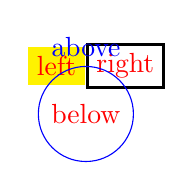
\begin{tikzpicture}[text = red]
\node[left, fill = yellow] at(0,0) {left};
\node[right, draw = black, line width =1pt] at(0,0) {right};
\node[above, text = blue] at(0,0) {above};
\node[below, draw = blue, circle] at(0,0) {below};
\end{tikzpicture}
```

如果你有一個很複雜的樣式,但又不是共通的,你可以利用`\tikzset{}`來將複雜的樣式定義成一個選項

```latex
\tikzset{mynode/.style = {
draw = gray!70!black,
line width = 0.8pt,
fill = blue!30,
rounded corners,
inner sep = 6pt, %文字與邊匡的距離
minimum width = 40pt,
minimum height = 20pt}
}
```

使用時只要用 `\node[mynode]` 即可

```latex
\begin{tikzpicture}[->, line width = 2pt]
\node[mynode] (1) at (0,0) {First Thing};
\node[mynode] (2) at (3,0) {Second Thing};
\node[mynode] (3) at (6,0) {Third Thing};
\draw (1)--(2);
\draw (2)--(3);
\end{tikzpicture}
```

這樣就方便許多了

###函數圖

畫函數一樣是使用`\draw ` 這個命令

```latex
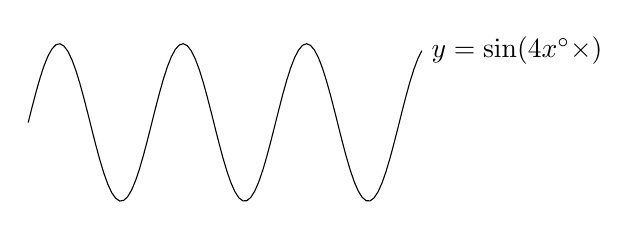
\begin{tikzpicture}
\draw[domain = 0:5, samples = 100] plot (\x,{sin(deg(\x*4))}) node[right] {$y=\sin(4x^\circ \times)$};
\end{tikzpicture}
```

domain 是我們要畫的區間,起點與終點要用冒號隔開,samples 決定圖形的精細程度,要特別注意的是需要運算的部分需要放在`{}`之間

![TikZ](TikZ)

上圖是可以使用的運算子,不過更複雜的函數圖形 TikZ 就很難畫出來了,所以下一篇會介紹 pgfplot 這個 package

\end{markdown}
\newpage
\begin{markdown}
#30天 LaTeX 挑戰 Day 22 pgfplots

------

pgfplots 是一個可以畫出複雜的三維圖表的強大 Package,需要注意的是這個 Package 是基於前面介紹過的 Ti*k*Z,所以在使用之前請記得要先使用 Ti*k*Z。

##簡介

在使用 pgfplots 之前我們需要先使用 tikzpicture 環境,之後再使用 pgfplots  提供的 axis 環境。

```latex
\begin{tikzpicture}
\begin{axis}
......
\end{axis}
\end{tikzpicture}
```

我們要將 pgfplots 提供的命令放在 axis 環境中,第一個要介紹的是 `\addplot[可選參數]{方程式}` 這個命令,大部分可選參數是與 Ti*k*Z 的可選參數相同,方程式則是與大部分程式語言的表達方式一樣。

```latex
\begin{tikzpicture}
\begin{axis}
\addplot[domain=-5:5, color=blue] {x^2};
\end{axis}
\end{tikzpicture}
```

使用完之後也請不要忘記在最後面加上 ;。

##二維圖形

###函數圖

第一個介紹的還是函數圖,簡單的範例上面展示過了,所以這裡會比較注重在介紹不同的可選參數。

```latex
\begin{tikzpicture}
\begin{axis}
\addplot[domain=-5:5, color=blue] {x^2};
\end{axis}
\end{tikzpicture}
```

這是上面所展示的陽春例子,我們可以在多加一個方程式讓他看起來好一點。

```latex
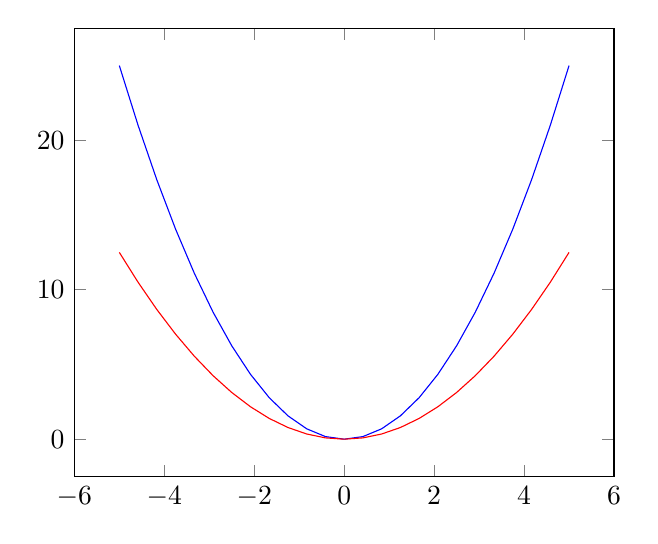
\begin{tikzpicture}
\begin{axis}
\addplot[domain=-5:5, color=blue] {x^2};
\addplot[domain=-5:5, color=red] {x^2/2};
\end{axis}
\end{tikzpicture}
```

可是這樣沒有標示難免會讓人搞混,所以我們可以利用 `\addlegendentry ` 加入註解。

```latex
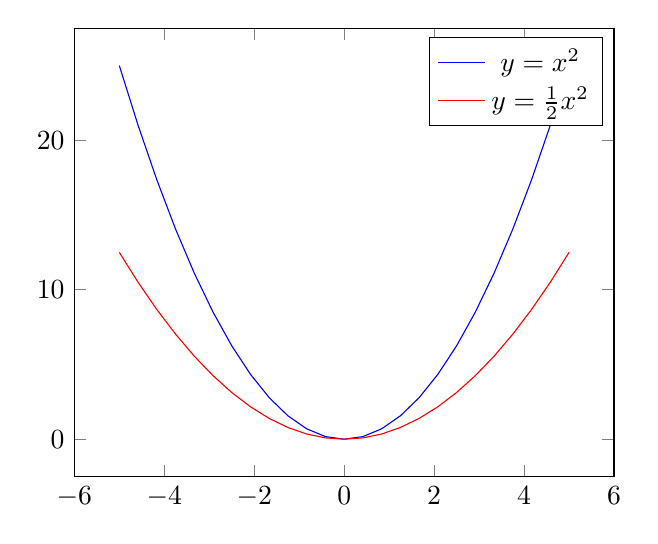
\begin{tikzpicture}
\begin{axis}
\addplot[domain=-5:5, color=blue] {x^2};
\addlegendentry{\(y=x^2\)}
\addplot[domain=-5:5, color=red] {x^2/2};
\addlegendentry{\(y=\frac{1}{2}x^2\)}
\end{axis}
\end{tikzpicture}
```

這樣就不會搞混了,如果今天想要用對數來當 x, y 軸的單位,pgfplots 也有提供 `\begin{semilogxaxis}` 與 `\begin{semilogyaxis}` 來解決這個問題。

```latex
\begin{tikzpicture}
\begin{semilogyaxis}
\addplot[domain=-10:10, color=blue, samples=1000] {log10(x)};
\end{semilogyaxis}
\end{tikzpicture}
```

有時候座標軸會不符合我們想要的樣式,這時可以利用 axis lines 來調整。

```latex
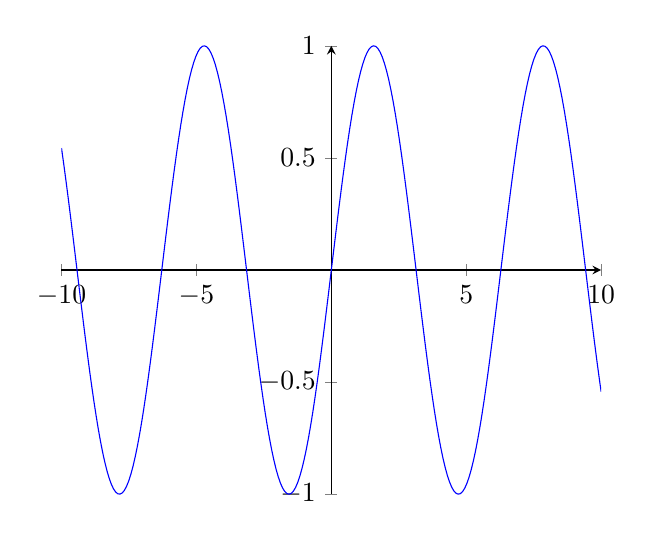
\begin{tikzpicture}
\begin{axis}[axis lines = middle]
\addplot[domain=-10:10, color=blue, samples=250] {sin(deg(x))};
\end{axis}
\end{tikzpicture}
```

\end{markdown}\newpage
\input{23拷貝}\newpage
\input{24拷貝}\newpage
\input{25拷貝}\newpage
\input{26拷貝}\newpage
\begin{markdown}
#30天 LaTeX 挑戰 Day 27 lualatex
\end{markdown}\newpage
\input{28拷貝}\newpage
\begin{markdown}
#30天 LaTeX 挑戰 Day 29 etoolbox

-------

倒數第二天了,今天要跟大家介紹 etoolbox 這個可以讓你編輯已有命令的 package。

##使用之前

因為這個 package 是讓你編輯已有命令,所以在編輯之前我們必須先找出命令的原始定義,LaTeX 提供了 `\show` 這個命令來協助我們,只要在 `\show `後面接上想要查詢的指令就在 .log 檔中看到命令的定義,除了利用`\show `查詢之外,我們也可以直接到檔案的原始碼尋找。

###



\end{markdown}\newpage
\begin{markdown}
#30天 LaTeX 挑戰 Day 30 繼續前行

-----

30 天的鐵人賽長跑來到了最後一天,今天就不再寫技術相關的內容了,而要來介紹哪裡可以找到更多關於 LaTeX 的資料,

##網頁

以下幾個網頁是我很推薦的資料來源

* CTAN
* Overleaf
* Stack Exchange

CTAN 是 Comprehensive TeX Archive Network 的縮寫,基本上只要是 TeX 有關的資料都會被收藏在此(LaTeX 當然也被包含在內),如果有什麼 package 或使用手冊想要找,甚至是自己寫了一個 package 想要與全世界的 TeX 使用者共享,只要到 CTAN 就對了。

Overleaf 不只提供了線上編譯 LaTeX 的服務,他們也為了推廣 LaTeX 寫了許多的技術文章,最棒的是他們的技術文章是為了初學者而設計的,所以不用怕看不懂,但想當然的內容是用英文寫的。

大部分人應該都聽過 Stack Exchange ,如果你有什麼問題想問,不仿先來這裡看看有沒有人問過。

##書籍

書籍有以下幾本

* The TeX book
* The Not So Short Introduction to LATEX2ε
* 簡單高效 LaTeX
* 大家來學 LaTeX

The TeX Book 是由高德納教授親自編寫的書籍,可以說是

\end{markdown}\newpage
\setlength{\parindent}{20pt}
\begin{markdown}
#30天 LaTeX 挑戰 Day 31 Beyond LaTeX

-------

30 天的挑戰終於過去了,我也算是用另一種方式成為了勇者,當初會想寫下這系列的文章可說全部都是意外,事情得要從一個地科作業開始說起,當時在寫地科作業的我正被「如何在 page 內加入數學方程式」而困擾著,於是我打開了 page 內建的插入方程式功能,只見一行大字出現在視窗內「請使用 mathml 或 LaTeX 來插入數學方程式」,這就是我遇見 LaTeX 的過程。

後來我就開始學習 LaTeX ,在學習的過程中我發現跟 LaTeX 有關的中文資料只有兩種,不是簡體字就是有一定年份的資料,除了這之外就全部都是英文資料了,雖然雙語能力固然重要,但沒有中文資料真的太慘了,所以我就下定決心要留點資料,那時剛好看到了鐵人賽,於是便下定決心要做這件事情。

\end{markdown}

\end{document}